\begin{pastexam}[label={px:ccu-110-swa-01}]{中正資工所甲組 110 學年度 第 3 題}
（單選）

(9\%) To find the articulation points in the graph below, start with constructing a
depth-first spanning tree by doing a depth-first search of the graph. Instead of choosing an
arbitrary vertex to start, your first vertex must be set to vertex A, and select the smallest
vertex in alphabetical order first when performing the depth-first search.

\begin{center}
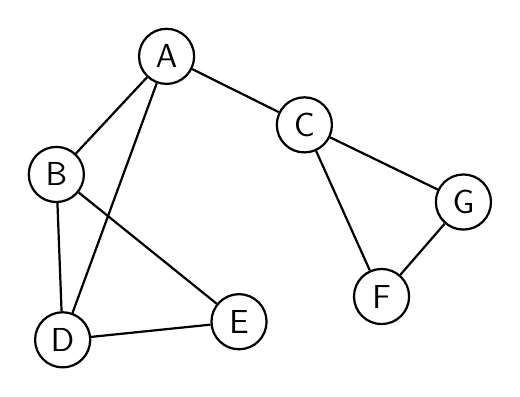
\begin{tikzpicture}[v/.style={circle,draw,thick,minimum size=7mm,inner sep=0pt,font=\sffamily\large},e/.style={thick}]
\node[v] (A) at (9.20,-17.95) {A};
\node[v] (B) at (7.80,-19.45) {B};
\node[v] (C) at (10.95,-18.82) {C};
\node[v] (D) at (7.88,-21.55) {D};
\node[v] (E) at (10.12,-21.32) {E};
\node[v] (F) at (11.93,-21.00) {F};
\node[v] (G) at (12.97,-19.80) {G};
\draw[e] (A) -- (B);
\draw[e] (A) -- (C);
\draw[e] (A) -- (D);
\draw[e] (B) -- (D);
\draw[e] (B) -- (E);
\draw[e] (D) -- (E);
\draw[e] (C) -- (F);
\draw[e] (C) -- (G);
\draw[e] (F) -- (G);
\end{tikzpicture}
\end{center}

\medskip
3.1 (2\%) (\quad) What are the edges of the depth-first spanning tree?

(a)~(A, B), (B, D), (D, E), (A, C), (C, F), (C, G)\\
(b)~(A, B), (A, D), (D, E), (A, C), (C, F), (F, G)\\
(c)~(A, B), (B, D), (B, E), (A, C), (C, F), (C, G)\\
(d)~(A, B), (A, C), (A, D), (D, E), (C, F), (C, G)\\
(e)~(A, B), (B, D), (D, E), (A, C), (C, F), (F, G)\\
(f)~None of the above

\medskip
3.2 (2\%) (\quad) What are the depth-first numbers (\textit{dfn}) of each vertex (in the order
of A, B, C, D, E, F, G), when performing the depth-first search on the graph above?

\begin{tabular}{@{}lll@{}}
(a)~(1, 2, 3, 4, 5, 6, 7) & (b)~(1, 5, 2, 6, 7, 3, 4) & (c)~(1, 2, 5, 3, 4, 6, 7) \\
(d)~(1, 4, 5, 2, 3, 7, 6) & (e)~(1, 3, 2, 7, 6, 5, 4) & (f)~None of the above
\end{tabular}

\medskip
3.3 (3\%) (\quad) What are the output value of the low function (i.e., \textit{low(v)}) for
each vertex (in the order of A, B, C, D, E, F, G) based on (3.1) and (3.2)?

\begin{tabular}{@{}lll@{}}
(a)~(1, 2, 1, 2, 2, 5, 5) & (b)~(1, 1, 5, 1, 2, 5, 5) & (c)~(1, 1, 5, 1, 1, 5, 5) \\
(d)~(1, 1, 5, 1, 4, 6, 7) & (e)~(1, 2, 5, 2, 2, 5, 5) & (f)~None of the above
\end{tabular}

\medskip
3.4 (2\%) (\quad) What are the articulation points in the graph?

\begin{tabular}{@{}lll@{}}
(a)~(A, C) & (b)~(B, C) & (c)~(A) \\
(d)~(A, B, C) & (e)~(A, E, G) & (f)~None of the above
\end{tabular}
\end{pastexam}

\begin{pastsoln}
答案：3.1 選 (e)；3.2 選 (c)；3.3 選 (b)；3.4 選 (a)。

題目的 dfn 就是資結書第~23.5~節割點演算法的 $d$（發現順序，從 $1$ 起）；$\mathit{low}$ 也用
那一節的定義：$\mathit{low}[u]$ 是 $d[u]$、$u$ 的子孫經由一條後向邊能回到的 $d[w]$、以及
子節點的 $\mathit{low}$ 三者的最小值，後向邊取 $d[w]$。

「先走字母小的」就是鄰接串列依字母排：
\begin{center}
$A\colon B, C, D$ \qquad $B\colon A, D, E$ \qquad $C\colon A, F, G$ \qquad $D\colon A, B, E$ \\
$E\colon B, D$ \qquad $F\colon C, G$ \qquad $G\colon C, F$
\end{center}
照資結書虛擬碼~23.3 從 $A$ 開始：
\begin{itemize}
\item $A$（$d = 1$）$\to B$（$2$）。 $B$ 的鄰居 $A$ 是父節點，跳過；$D$ 還沒發現，$B \to D$（$3$）。
\item $D$ 的鄰居 $A$ 已發現、不是父節點，後向邊 $\{D, A\}$；$B$ 是父節點；$E$ 還沒發現，
$D \to E$（$4$）。
\item $E$ 的鄰居 $B$ 是祖先，後向邊 $\{E, B\}$；$D$ 是父節點。 $E$ 完成，接著 $D$、$B$ 完成。
\item 回到 $A$，下一個鄰居 $C$ 還沒發現，$A \to C$（$5$）；$C \to F$（$6$）；$F$ 的鄰居 $C$ 是
父節點，$G$ 還沒發現，$F \to G$（$7$）；$G$ 的鄰居 $C$ 是祖先，後向邊 $\{G, C\}$；$F$ 是父節點。
\item 回到 $C$，鄰居 $G$ 已經發現過（是子孫），略過。 回到 $A$，最後一個鄰居 $D$ 已經完成，
略過。
\end{itemize}

\begin{center}
\begin{tikzpicture}[v/.style={circle,draw,thick,minimum size=7mm,inner sep=0pt,font=\sffamily},
  tr/.style={very thick}, bk/.style={thick,dashed}, lab/.style={font=\small,inner sep=1pt}]
\node[v] (A) at (0,0) {A};
\node[v] (B) at (-1.5,-1.2) {B};
\node[v] (D) at (-1.5,-2.4) {D};
\node[v] (E) at (-1.5,-3.6) {E};
\node[v] (C) at (1.5,-1.2) {C};
\node[v] (F) at (1.5,-2.4) {F};
\node[v] (G) at (1.5,-3.6) {G};
\draw[tr] (A) -- (B); \draw[tr] (B) -- (D); \draw[tr] (D) -- (E);
\draw[tr] (A) -- (C); \draw[tr] (C) -- (F); \draw[tr] (F) -- (G);
\draw[bk] (D) to[bend right=35] (A);
\draw[bk] (E) to[bend right=45] (B);
\draw[bk] (G) to[bend left=45] (C);
\node[lab,left=2pt of A] {$1/1$};
\node[lab,left=2pt of B] {$2/1$};
\node[lab,left=2pt of D] {$3/1$};
\node[lab,left=2pt of E] {$4/2$};
\node[lab,right=2pt of C] {$5/5$};
\node[lab,right=2pt of F] {$6/5$};
\node[lab,right=2pt of G] {$7/5$};
\end{tikzpicture}
\end{center}
上圖粗線是樹邊、虛線是後向邊，頂點旁邊寫 $d/\mathit{low}$。

\textbf{3.1} 樹邊是 $(A, B)$、$(B, D)$、$(D, E)$、$(A, C)$、$(C, F)$、$(F, G)$，選 (e)。 其他選項：
(a)、(c)、(d) 有 $(C, G)$，但 $G$ 是從 $F$ 發現的（$C$ 的串列裡 $F$ 在 $G$ 前面，走到 $F$ 時 $G$
還沒發現）；(b)、(d) 有 $(A, D)$，但 $D$ 在 $A$ 看到它之前就由 $B$ 發現了；(c) 有 $(B, E)$，但
$E$ 是從 $D$ 發現的。 (e) 正確，(f) 不選。

\textbf{3.2} 依發現順序 $A = 1$、$B = 2$、$D = 3$、$E = 4$、$C = 5$、$F = 6$、$G = 7$。 依
$A, B, \ldots, G$ 排是 $(1, 2, 5, 3, 4, 6, 7)$，選 (c)。 (a) 是把字母順序當成發現順序；(b)、(d)、
(e) 都不是從 $A$ 先走 $B$ 的結果，例如 (b) 的 $d[B] = 5$ 表示先走完 $C$ 那一邊，(d)、(e) 的
$d[D] < d[B]$ 表示先走 $D$。

\textbf{3.3} 從葉節點往上算：

\begin{center}
\small
\begin{tabular}{ccccl}
\toprule
$u$ & $d$ & 子節點 & 後向邊到 & $\mathit{low}$ \\
\midrule
$E$ & 4 & — & $B$ & $\min(4, d[B]) = 2$ \\
$D$ & 3 & $E$ & $A$ & $\min(3, d[A], \mathit{low}[E]) = \min(3, 1, 2) = 1$ \\
$B$ & 2 & $D$ & — & $\min(2, \mathit{low}[D]) = 1$ \\
$G$ & 7 & — & $C$ & $\min(7, d[C]) = 5$ \\
$F$ & 6 & $G$ & — & $\min(6, \mathit{low}[G]) = 5$ \\
$C$ & 5 & $F$ & — & $\min(5, \mathit{low}[F]) = 5$ \\
$A$ & 1 & $B, C$ & — & $1$ \\
\bottomrule
\end{tabular}
\end{center}

依 $A, \ldots, G$ 排是 $(1, 1, 5, 1, 2, 5, 5)$，選 (b)。 其他選項都至少錯一格：(a)、(e) 的
$\mathit{low}[B] = 2$ 漏掉了子孫 $D$ 的後向邊 $\{D, A\}$，(a) 的 $\mathit{low}[C] = 1$ 也不對，
$C$ 那一邊沒有邊回到 $A$；(c) 的 $\mathit{low}[E] = 1$，但 $E$ 沒有子節點，唯一的後向邊回到
$d[B] = 2$；(d) 的 $\mathit{low}[E] = 4$、$\mathit{low}[F] = 6$、$\mathit{low}[G] = 7$ 沒有算後向邊
$\{E, B\}$、$\{G, C\}$。

\textbf{3.4} 根 $A$ 在 DFS 樹裡有兩個子節點 $B$、$C$，是割點（資結書定理~23.8）。 非根的頂點用
資結書定理~23.9：$u$ 是割點若且唯若它有一個子節點 $v$ 使 $\mathit{low}[v] \ge d[u]$。
\begin{itemize}
\item $C$ 的子節點 $F$ 有 $\mathit{low}[F] = 5 \ge d[C] = 5$，$C$ 是割點。
\item $B$ 的子節點 $D$ 有 $\mathit{low}[D] = 1 < 2$；$D$ 的子節點 $E$ 有 $\mathit{low}[E] = 2 < 3$；
$F$ 的子節點 $G$ 有 $\mathit{low}[G] = 5 < 6$。 $B$、$D$、$F$ 都不是割點。
\item $E$、$G$ 是葉節點，不是割點。
\end{itemize}
割點是 $A$、$C$，選 (a)。 直接檢查也對得上：拿掉 $A$，$\{B, D, E\}$ 和 $\{C, F, G\}$ 分開；拿掉
$C$，$\{F, G\}$ 和其他頂點分開；拿掉其他任何一個頂點，剩下的圖都還連通。 (b)、(d) 含 $B$，(c) 漏了
$C$，(e) 含葉節點 $E$、$G$，都錯。
\end{pastsoln}
